A binned maximum likelihood fit is performed on the $\etalj$ distribution to determine the signal cross section. The fit is implemented with the statistical framework \texttt{theta}. Different background processes with the same behavior are grouped together in order to reduce the impact of yield uncertainties of the individual process. Background contributions from top quarks, namely $\ttbar$ pair production and tW-channel single top quark production ($s$-channel single top quark production is neglected), are grouped together in the top background category, whereas \wjets and \zjets defines the electroweak background category. A third background category consists of QCD events, its contribution is derived from the procedure described in Section~\ref{sec:qcd} and kept fixed. The fit is done simultaneously in the signal enriched 2J1T region and the 3J2T region. The latter one is dominated by $\ttbar$ events, which helps to reduce the uncertainty of the top background component. Simulation studies showed that the requirement of a second b-tag leads to vanishing QCD-contribution in the 3J2T region, and therefore this background is neglected in this region. For all but the QCD background templates from MC simulation are used for the fit. The QCD template is derived from data as described in Section~\ref{sec:qcd}.

%The result of the fit is estimated using pseudo-data generated by the rejection sampling technique, where the probability shape is derived from the stacked Monte Carlo histograms. It was observed in different analyses during Run~I that the \wjets process was not well-modeled in Monte Carlo simulations, especially the heavy flavor component. Since this effect will also be observable in our analysis due to our selection the \wjets template is scaled by a factor of 1.8.

The free parameters of the fit are the scale factors of the $t$-channel signal process and the top/electroweak background categories. Both background scale factors are constrained by a Gaussian prior with an uncertainty of 20\% for the top background and 30\% for the electroweak background. The scale factors are defined as:

\begin{equation}
S_i = \frac{N_i}{N_i ^{\text{exp}}}
\label{eq:scalef}
\end{equation}

where $N_i$ is the number of events after the fit, $N_i ^{\text{exp}}$ the expected number of events and $i$ the process category. The fit is performed with a cut on the transverse \PW~boson mass ($\mtw > 50~\GeV$) and inside the top mass window ($130 < m_{\text{top}} < 225~\GeV$). Table~\ref{tab:fitresult} shows the results obtained from the fit.

\begin{table}[!h]
\begin{center}
\caption{\label{tab:fitresult} Scale factors from the fit for the signal process and the background categories.}
\begin{tabular}{c|c}
Process & Scale factor \\
\hline
$t$-channel   & 1.26 $\pm$ 0.45  \\
top        & 1.03 $\pm$ 0.10 \\ 
electroweak    & 1.02 $\pm$ 0.27  \\
\end{tabular}
\end{center}
\end{table} 

The significance of the signal process was found to be 2.88~$\sigma$. All fitted distributions are shown in Figure~\ref{fit:result}.

\begin{figure}[!h]
\begin{center}
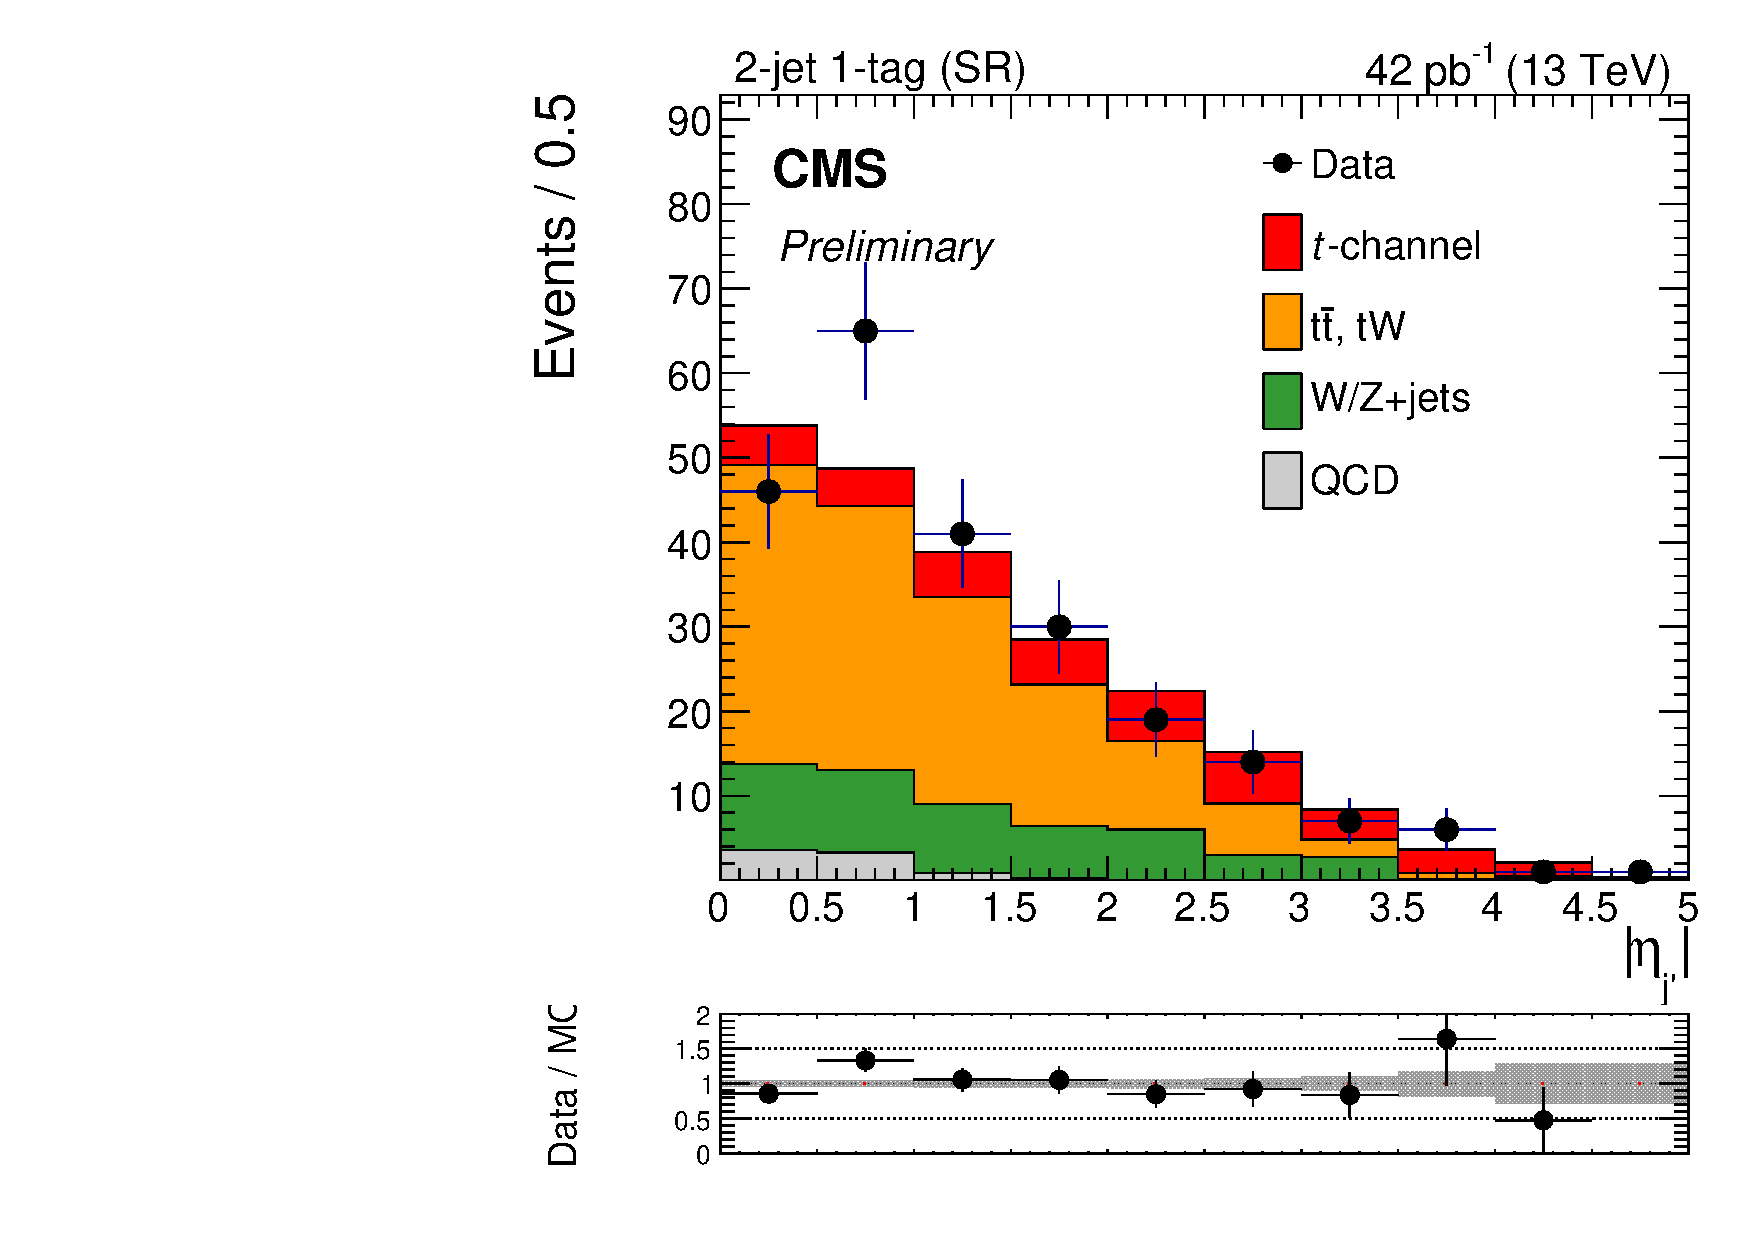
\includegraphics[angle=00,width=0.45\textwidth]{figures/postfit2D_MVA_mu2j1t.pdf}
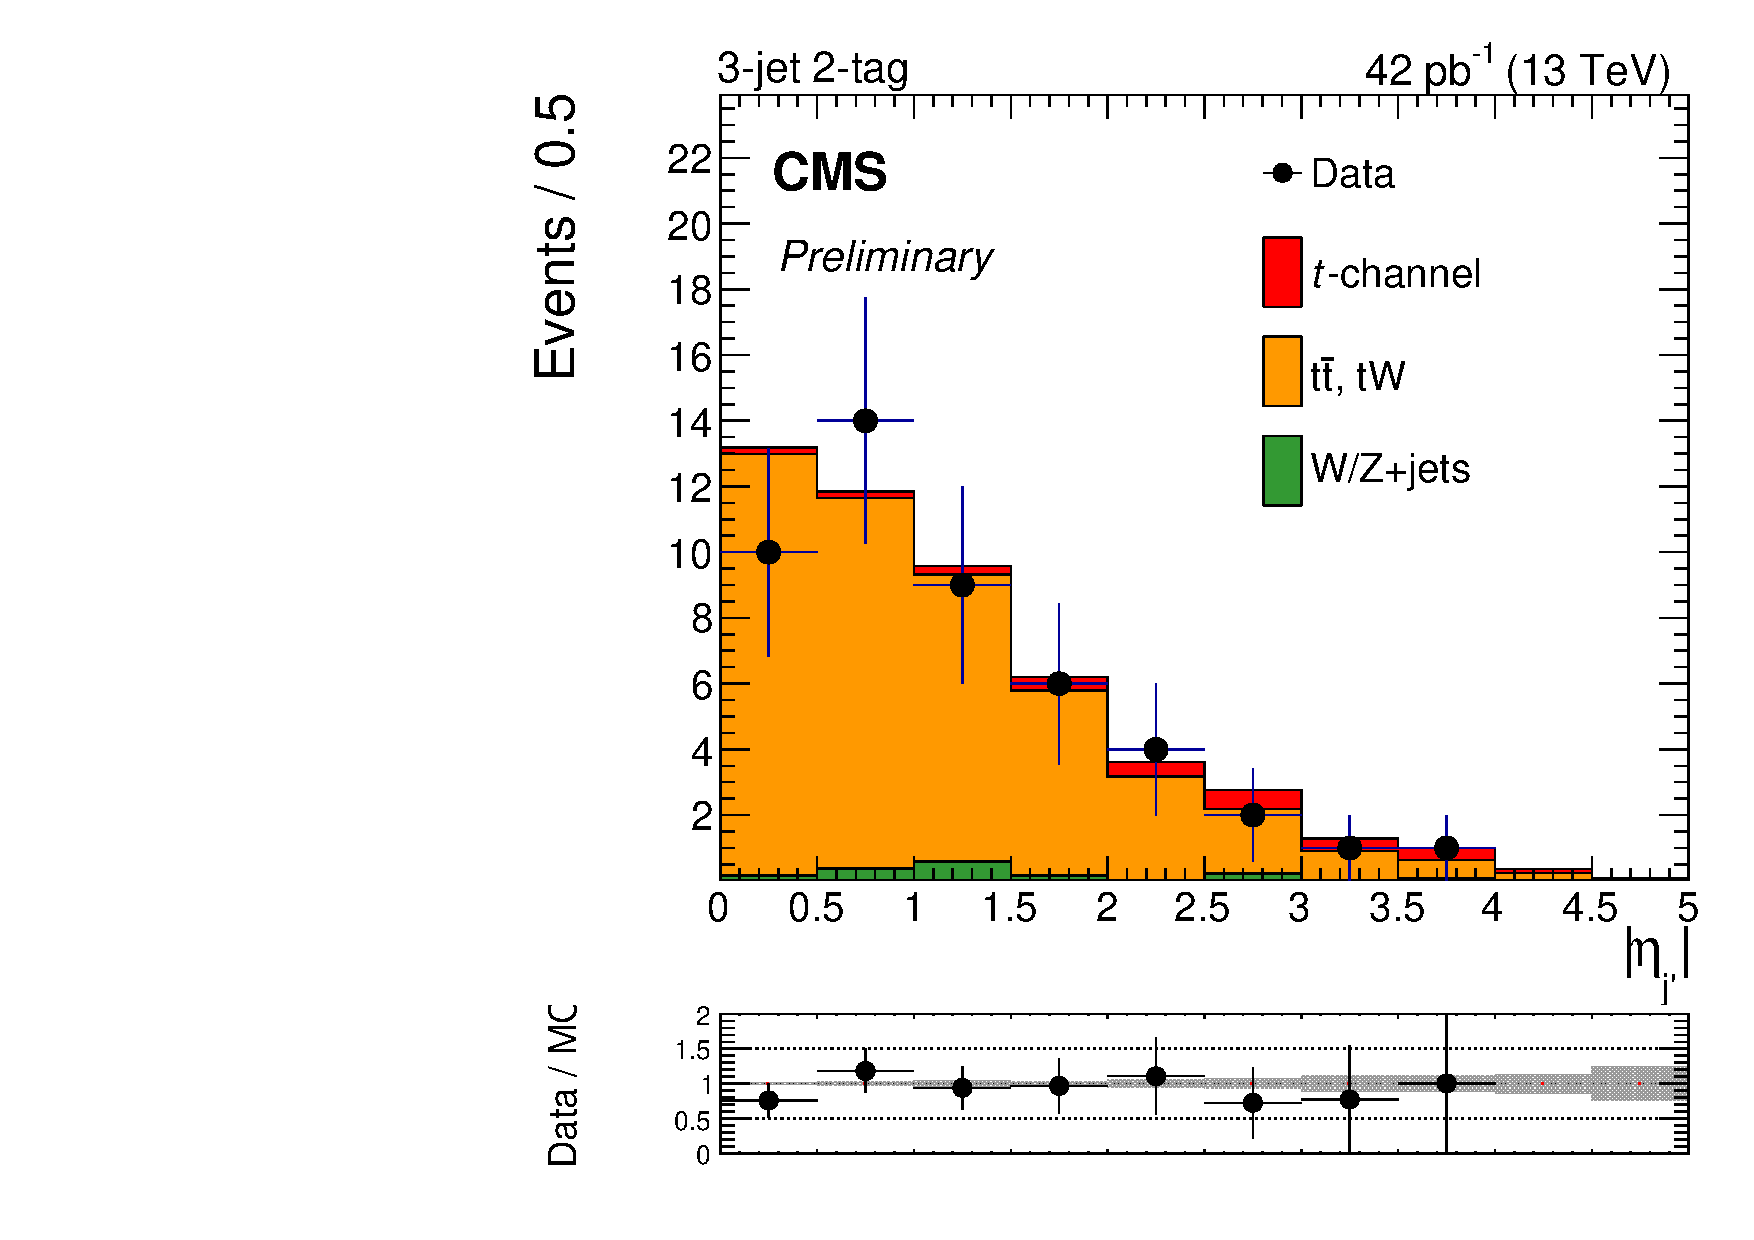
\includegraphics[angle=00,width=0.45\textwidth]{figures/postfit2D_MVA_mu3j2t.pdf}
\caption{\label{fit:result} Fitted $\etalj$ distributions in the 2J1T and 3J2T region normalized to the yields obtained from the fit.}
\end{center}
\end{figure}

Figure~\ref{fit:scaled} shows the distribution of the light jet pseudorapidity $\eta_{j'}$, the reconstructed top quark mass $m_{\text{top}}$ and the angle between the charged lepton and the light jet in the rest frame of the top quark $\cos(\theta^*)$ in the 2J1T region without the cut on the top mass. The latter two distributions for the signal-enriched forward-region only ($\eta_{j'} > 2.5$) can be found in Appendix~\ref{app:forward}.

\begin{figure}[!h]
\begin{center}
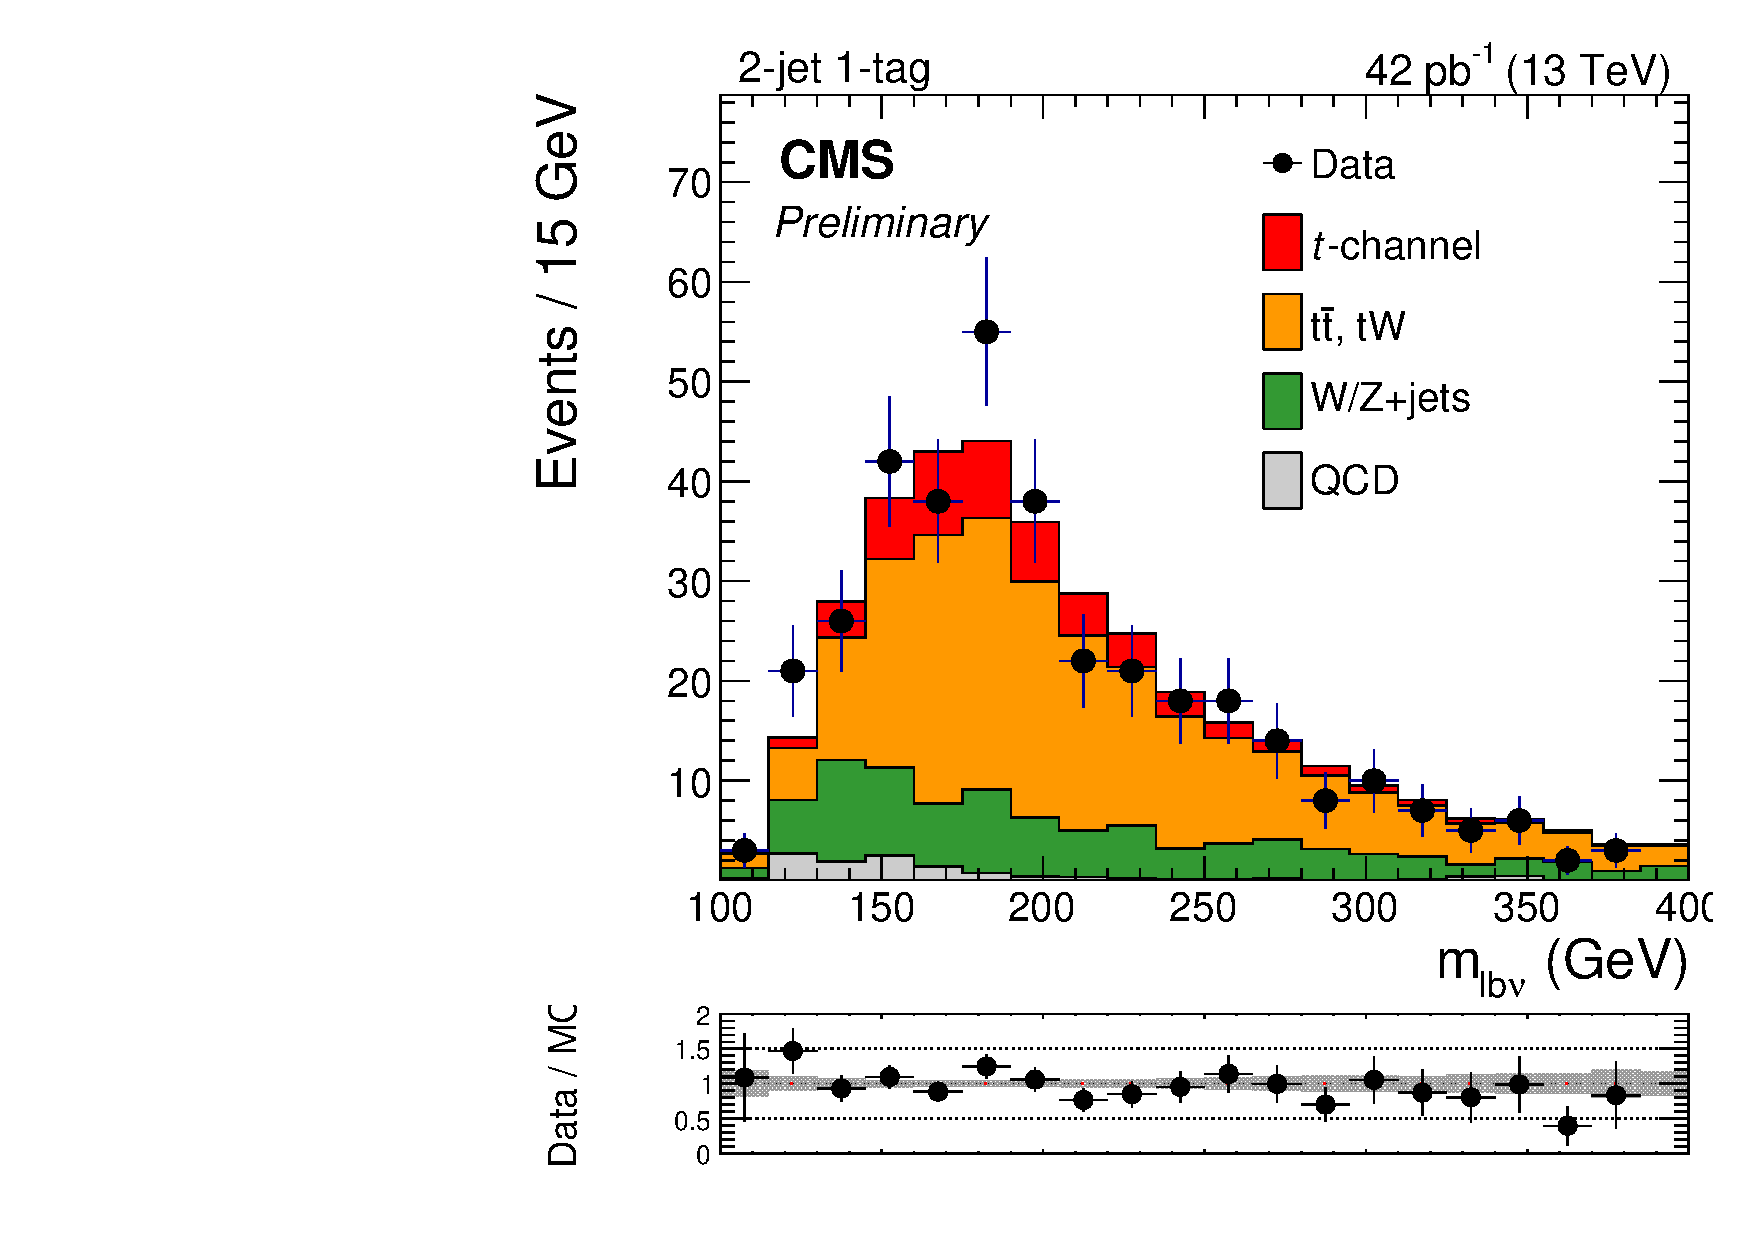
\includegraphics[angle=00,width=0.4\textwidth]{figures/postfit_topm_incl.pdf}
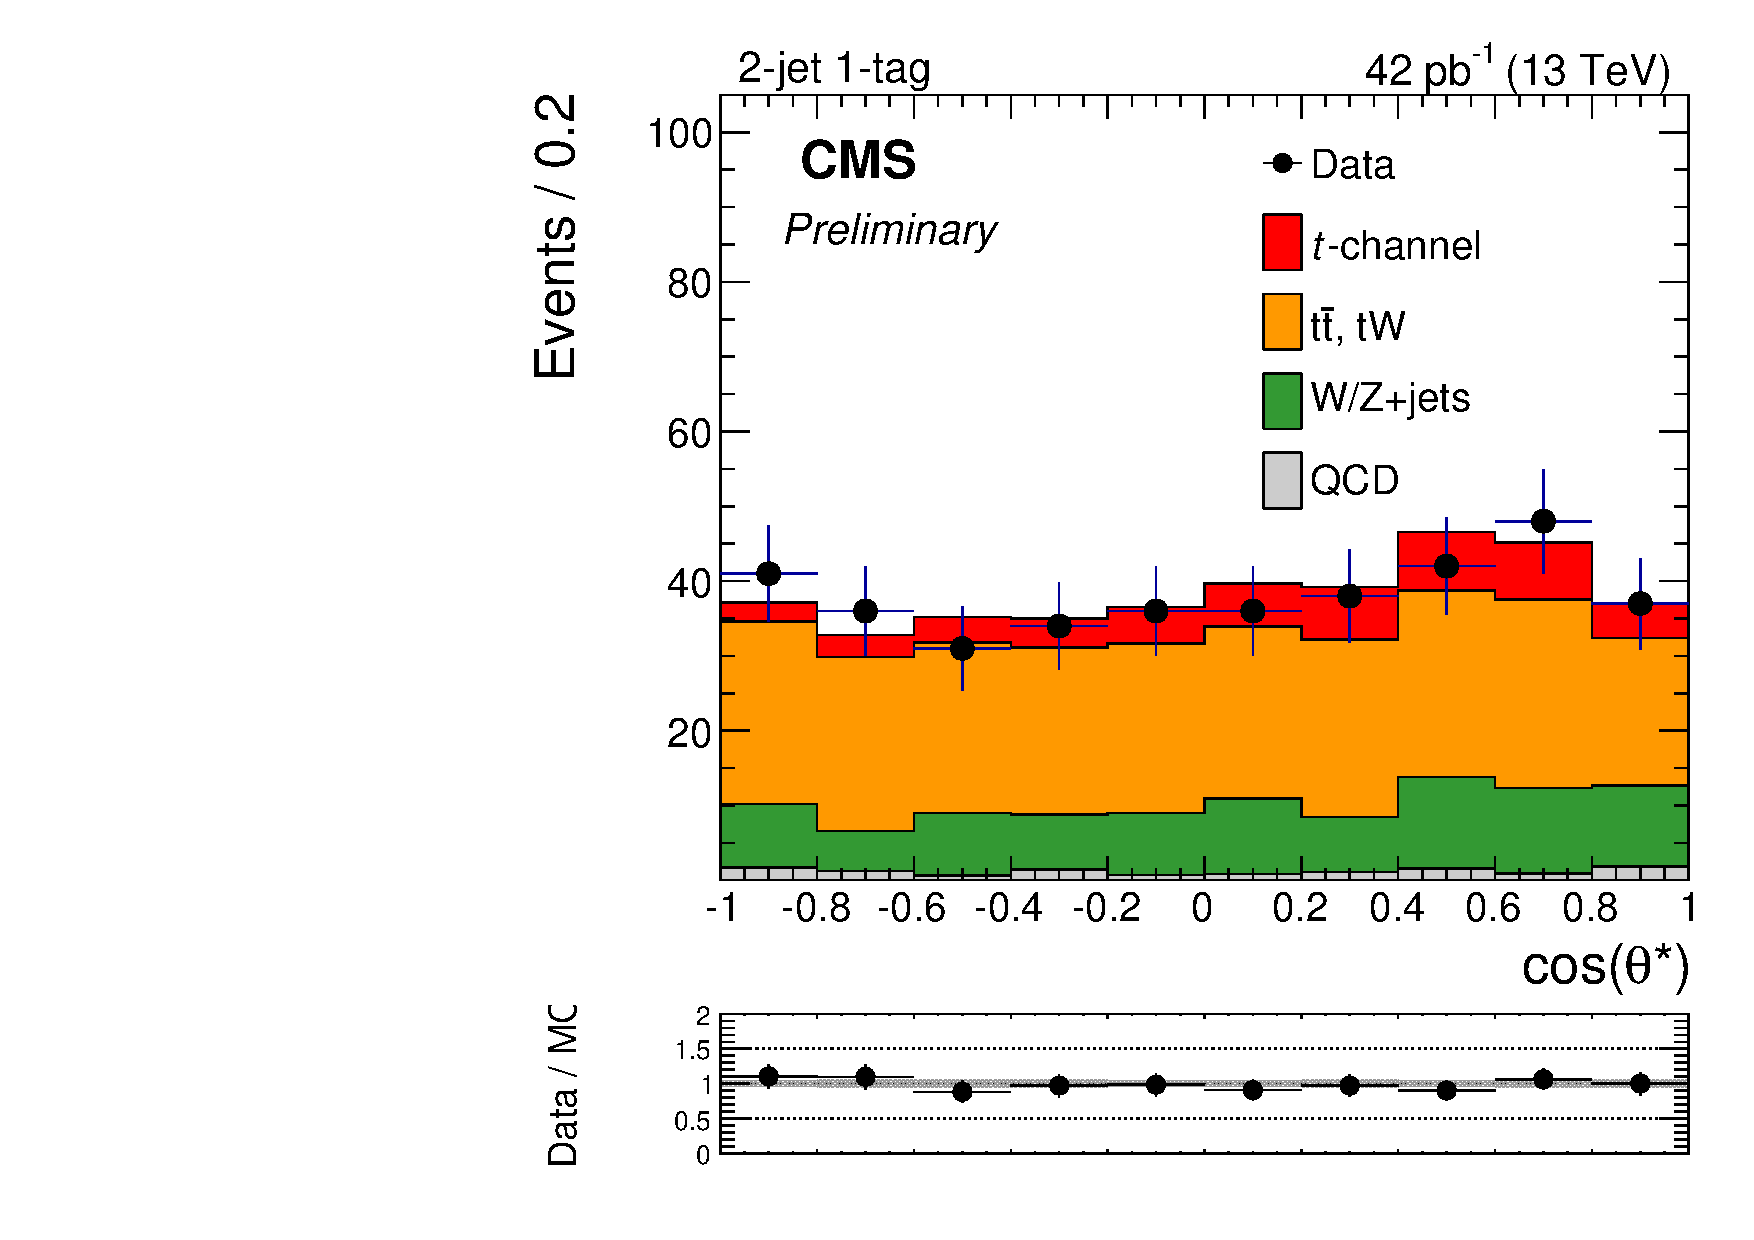
\includegraphics[angle=00,width=0.4\textwidth]{figures/postfit_costhetastar_incl.pdf}
\caption{\label{fit:scaled} Distribution of $m_{\text{top}}$ and $\cos(\theta^*)$ in the 2J1T region. The MC templates are scaled to the result of fit.}
\end{center}
\end{figure}

The single top quark $t$-channel cross section is then calculated with the formula:

\begin{equation}
\sigma_t = \frac{N_{\mathrm{s}}}{\epsilon \cdot \mathcal{B}(\mathrm{t}\to\ell\nu b) \cdot L}
\label{eq:crosssection}
\end{equation}

where $N_{\mathrm{s}}$ is the number of signal events, $\epsilon$ the selection efficiency, $\mathcal{B}(\mathrm{t}\to\ell\nu b)\, = \, 0.324$~\cite{pdg} the overall leptonic branching ratio and $L$ the integrated luminosity.
 %The sensitivity of the measurement has also been computed.
%The free parameters of the fit are the yields of the $t$-channel signal, the electroweak backgrounds (W/Z+jets, Diboson), 
%and the top backgrounds ($\ttbar$, tW, and $s$ single top channels), while the QCD is costrained to the value obtained 
%from the control samples in data and the corresponding uncertainty propagated as systematic uncertainty. 
%The background components defined above in groups are treated separately in the fit
%in order to reduce the effect of the uncertinties of the individual yield SM predictions.
%The different $\etalj$ distributions of the groups of backgrounds considered
%have sufficiently different shapes to allow a separation in the fit to the distribution in data.

%We define the following extended likelihood function, for both the muon and electron channels:
%\begin{equation}
%\label{eq:likelihood}
%\footnotesize{
%\begin{split}
%L_c&(N_{\mathrm{s_c}},  N_{\mathrm{b_c}} | \eta_1, ..., \eta_n)  = \\ 
%& = \Pai_{c} e^{-(N_{s_c} + N_{\mathrm{EWK_c}} + N_{\mathrm{top_c}} + N_{\mathrm{QCD_c}})} \,\prod_{k=1}^n 
% \bigg(N_{\mathrm{s_c}}\cdot P_{\mathrm{s_c}}(\eta_k)+ N_{\mathrm{EWK_c}} \cdot P_{\mathrm{EWK_c}}(\eta_k) + N_{\mathrm{top_c}} \cdot P_{\mathrm{top_c}}(\eta_k)+ N_{\mathrm{QCD_c}}\cdot P_{\mathrm{QCD}}(\eta_k_c)\bigg)
%\end{split}
%}
%\end{equation}
%$N_{\mathrm{s}}$, $N_{\mathrm{EWK}}$, $N_{\mathrm{top}}$, $N_{\mathrm{QCD}}$ are the yields of signal and background components, 
%$n$ is and number of observed events,  and $P_{\mathrm{s}}$, $P_{\mathrm{b}}$, b=(EWK, top, QCD), are the PDFs for the signal and 
%the different background components. $P_{\mathrm{s}}$ is taken from Monte Carlo. 
%$P_{\mathrm{top}}$ is taken correcting the MC shape by the data-driven, bin by bin scale factors derived in Sec.~\ref{sec:ttbar}.
%The index $c$ is used to indicate the three different likelihoods defined for positively, negatively charged leptons, or leptons where no selection on the charge is performed. 
%%Figure ~\ref{fig:remodeledEtas}(a) shows the comparison between \tt shape from MC (continuous line) and the data-driven shape (triangles).
%%The $EWK$ is consistently derived taking into account the data-driven shape of \tt.
%%The procedure to extract the background is ar to the one in ~
%%Figure ~\ref{fig:remodeledEtas}(b) shows the $EWK$ shape taken from simulation (red line),
%the one extracted with the data driven technique described in Sec~\ref{sec:wjets} using ttbar from simulation (blue line),
% and ttbar from the data driven technique (triangles).
%Figure \ref{fig:remodeledEtas} show the data driven shapes for \tt and \wjets which are used in the fit.
%
%	\begin{figure}[h]
%	  \begin{center}
%	    \subfigure[]{
%	    \includegraphics[width=0.48\textwidth]{figures/2J1T/2J_1T_TopShapeDD.png}}
%	    \subfigure[]{
%	    \includegraphics[width=0.48\textwidth]{figures/2J1T/2J_1T_EWKShapeDD.png}}
%%	    \caption{\label{fig:remodeledEtas}{ \etalj of (a) \tt and (b) \wjets extracted using data driven techniques in the 2-jets 1-tag signal region
%	    compared to MC expectations.}}
%	  \end{center}
%	\end{figure}

%Since \topMass and \etalj~ are weakly correlated variables (we estimated, with Monte Carlo, a correlation of 1.5\% for signal and 2\% for the overall
%background), we factorize $P_s$ and $P_{b=ewk,top,qcd}$ into the product of separated functions:
%$P_s = F_s(\eta)$ and $P_{b=ewk,top,qcd} = F_b(M_{lb\nu}^*) \cdot G_b(\eta)$.
%$N_{\mathrm{s}}$ and the various $N_{\mathrm{b}}$ are determined from the fit assuming
%the PDF to be fixed, taken either from simulation or form control samples in data, as discussed in the previous sections. 
%In the following two paragraph the two different fits performed to extract the inclusive $t$-channel cross section and the 
%$t$-channel charge ratio are described in the detail.

% REDUNDANT
%
% To be more specific, the background term in Eq.~(\ref{eq:likelihood}) is given by:
% \begin{equation}
% N_{\mathrm{b}} \cdot P_{\mathrm{b}}(\eta) = \sum_i N_{b_i} \cdot G_{b_i}(\eta) 
% \label{eq:pb}
% \end{equation}
% where $i$ runs over all the backgrounds (whose relative normalizations are taken from Monte Carlo) which compose the $b$ template.
%\subsection{Inclusive cross section fit}
%It is convenient to define the signal strength $S_{\mathrm{s}}$,  the EWK strength $S_{\mathrm{EWK}}$, and the top strength $S_{\mathrm{top}}$ as the ratios of the measured and expected yields  $N_{i}$ and $N_{i}^{\mathrm{exp}}$:
%\begin{eqnarray}
%\label{eq:strength}
%S_{i} = N_{i}/N_{i}^{\mathrm{exp}}\,,i=\mathrm{s},\,\mathrm{EWK},\,\mathrm{top}\,.
%\end{eqnarray}
%Whenever the fit results will be expressed in terms of $S_i$, they will refer to 
%Tab.~\ref{tab:2J1T} for $N_{i}^{\mathrm{exp}}$.
%The fitted $\etalj$ distributions are shown in Fig.~\ref{fig:fits_tot}.
%The fit results are the following:
%
%\begin{eqnarray}
%\label{eq:fitresults_s_tot}
%S_{\mathrm{s}} = \totmus \pm \totmustatss& S_{\mathrm{EWK}}  = \totmuewkmu \pm \totmustatsewkmu & S_{\mathrm{top}} = \totmutop \pm \totmustatstop  \quad\quad \text{(muons)}\,.      \nonumber \\
%S_{\mathrm{s}} = \toteles \pm \totelestatss & S_{\mathrm{EWK}}  = \toteleewkele \pm \totelestatsewkele & & S_{\mathrm{top}} = \toteletop \pm \totelestatstop  \quad\quad \text{(electrons)}\,.      \nonumber \\
%\end{eqnarray}
%
%\begin{eqnarray}
%\label{eq:fitresults_muele_s_tot}
%S_{\mathrm{s,-}} = \totmueles \pm \totmuelestatss  & S_{\mathrm{EWK,\mu-}}  = \totmueleewkmu \pm \totmuelestatsewkmu \nonumber \\
% S_{\mathrm{EWK,e}} = \totmueleewkele \pm \totmuelestatsewkele  & S_{\mathrm{top}} = \totmueletop \pm \totmuelestatstop \quad\quad \text{(muons+electrons)}\,,   \nonumber\\
%\end{eqnarray}
%
%\begin{figure}[!h]
%\begin{center}
%	    \subfigure[]{
%\includegraphics[angle=00,width=0.48\textwidth]{figures/SR1etaNoVeto10BinsTTFitFixRemodelConstrMuStack.pdf}}
%	    \subfigure[]{
%\includegraphics[angle=00,width=0.48\textwidth]{figures/SR1etaNoVeto10BinsTTFitFixRemodelConstrEleStack.pdf}}\\
%	    \caption{\label{fig:fits_tot}{} Fitted $\etalj$ distribution for muons(a) and electrons(b), normalized to the yields obtained from the combined fit to the total cross section. }
%\end{center}
%\end{figure}
%
%
%\subsection{top/antitop ratio fit}
%The parameters of the fit are defined as relative strengths.
%The absolute normalizations for samples with the negatively charged leptons $S_{\mathrm{s,-}}$, $S_{\mathrm{EWK_{\mu},-}}$, $S_{\mathrm{EWK_{e},-}}$, and for the top background $S_{\mathrm{top}}$ are defined in the same way as in as in Eq. ~\ref{eq:strength}. 
%In addition, we fit the ratio strengths for the signal and the EWK component of the background $S_{\mathrm{R,s}}$, $S_{\mathrm{R,EWK}}$, 
%adopting the following definition:
%\begin{eqnarray}
%\label{eq:strength}
%S_{R,i} = R^{+/-}_{i}/R^{+/-}_{i}^{\mathrm{exp}}\,,i=\mathrm{s},\,\mathrm{EWK},\,\mathrm{top}\,,\\
%R^{+/-} = N^{+}/N^{-}\,.
%\end{eqnarray}
%The EWK component of muons and electrons is left floating and we fit the ratio $R_{EWK}$ simultaneously.
%The results of the fits, in the muon and electron channels, and with the simultaneous fit of the two are:
%
%\begin{eqnarray}
%\label{eq:fitresults_s_ch}
%S_{\mathrm{s,-}} = \chmusminus \pm \chmustatssminus & S_{\mathrm{s,ratio}} = \chmusratio \pm \chmustatssratio & S_{\mathrm{EWK,-}}  = \chmuewkmuminus \pm \chmustatsewkmuminus\, \nonumber \\
%S_{\mathrm{EWK,ratio}}  = \chmuewkratio \pm \chmustatsewkratio & S_{\mathrm{top}} = \chmutop \pm \chmustatstop  \quad\quad \text{(muons)}\,.      \nonumber \\
%S_{\mathrm{s,-}} = \chelesminus \pm \chelestatssminus & S_{\mathrm{s,ratio}} = \chelesratio \pm \chelestatssratio & S_{\mathrm{EWK,-}}  = \cheleewkeleminus \pm \chelestatsewkeleminus\, \nonumber \\
%S_{\mathrm{EWK,ratio}}  = \cheleewkratio \pm \chelestatsewkratio & S_{\mathrm{top}} = \cheletop \pm \chelestatstop  \quad\quad \text{(electrons)}\,.      \nonumber \\
%S_{\mathrm{s,-}} = \chmuelesminus \pm \chmuelestatssminus & S_{\mathrm{s,ratio}} = \chmuelesratio \pm \chmuelestatssratio\,   \nonumber \\
% S_{\mathrm{EWK,mu-}}  = \chmueleewkmuminus \pm \chmuelestatsewkmuminus & S_{\mathrm{EWK,e-}}  = \chmueleewkeleminus \pm \chmuelestatsewkeleminus \nonumber\,       \nonumber \\
% S_{\mathrm{EWK,ratio}}  = \chmueleewkratio \pm \chmuelestatsewkratio & S_{\mathrm{top}} = \chmueletop \pm \chmuelestatstop  \quad\quad \text{(muons+electrons)}\,.      \nonumber \\
%\end{eqnarray}
%
%The final result taking into account all scale factors for $\wjets$ charge asymmetry is the following:
%\begin{eqnarray}
%\label{eq:fitreults_wasym_s}
%R_{\wjets , \mu} = 1.06 \pm 0.06 \text{(muons)}\,.      \nonumber \\
%R_{\wjets , e} = 1.18 \pm 0.13 \text{(electrons)}\,.      \nonumber \\
%R_{\wjets , \mu + e} = 1.13 \pm 0.07 \text{(combined)}\,.      \nonumber \\
%\end{eqnarray}
%The numbers expected from the simulation are $R_{\wjets , \mu } = 1.35$,$R_{\wjets , e } = 1.17$, $R_{\wjets , \mu + e } = 1.27$ 
%but they have to be taken with care as this is critically dependent on the jet flavour composition and 
%on the phase space of the measurement, also it shown in tables ~\ref{tab:WAsymMu},~\ref{tab:WAsymEle},~\ref{tab:WAsymMu1J1T},~\ref{tab:WAsymEle1J1T}.
%
%The propagation of systematics uncertainties on jet flavour composition is thus not negligible with respect to the statistical uncertainty, and should be object of further appropriate studies.
%It has to be noted that $S_{\mathrm{EWK,-}}$ is expressed with respect to the data-driven prediction described in the detail in Sec. ~\ref{sec:systs}. 
%
%%We also perform a simultaneous fit in the muon and electron channels. In this case
%%in order to reduce the assumptons the EWK backgrounds, the EWK components are not assumed to be identical for electrons and muons, while
%%the other fit parameters are constrained to the same value.
%%The signal yield from the combined fit is:
%
%
%\begin{eqnarray}
%\label{eq:fitresults_comb_n}
%N_{\mathrm{s}} = \nevents \pm \neventserror &  \quad\quad \text{(combined)}\,,  \nonumber 
%\end{eqnarray}
%and the fitted signal strenghts are:
%\begin{eqnarray}
%\label{eq:fitresults_s}
%\qquad S_{\mathrm{s}} = \signalstrengthmu \pm \signalstrengthmustats \nonumber   & \qquad S_{\mathrm{EWK}}(\mu)  = \ewkstrengthmu \pm \ewkstrengtherrormu \nonumber  \qquad S_{\mathrm{top}} = \topstrengthmu \pm \topstrengtherrormu  \nonumber \\
%\end{eqnarray}%
%\begin{eqnarray}
%\label{eq:fitresults_comb_n}
%N_{\mathrm{s}} = \nevents \pm \neventserror &  \quad\quad \text{(combined)}\,,  \nonumber 
%\end{eqnarray}
%and the fitted signal strenghts are:
%\begin{eqnarray}
%\label{eq:fitresults_s}
%S_{\mathrm{s}} = \signalstrengthmu \pm \signalstrengthmustats \quad &  S_{\mathrm{EWK}}(\mu)  = \ewkstrengthmu \pm \ewkstrengthmuerror \nonumber \\ 
%S_{\mathrm{EWK}}(\mathrm{e}) = \ewkstrengthbis \pm \ewkstrengthbiserror \quad\quad &  S_{\mathrm{top}} = \topstrength \pm \topstrengtherror \quad\quad \text{(combined)}\,. \nonumber 
%\end{eqnarray}
%\begin{figure}[!h]
%\begin{center}
%	 %   \subfigure[]{
%%\includegraphics[angle=00,width=0.8\textwidth]{figures/xsection/SR1etaNoVeto10BinsTTFitFullRemodelMuStack.pdf}}
%	    \subfigure[]{
%\includegraphics[angle=00,width=0.48\textwidth]{figures/SR1etaNoVeto10BinsTTFitFixRemodelConstrMuStack_Plus.pdf}}
%	    \subfigure[]{
%\includegraphics[angle=00,width=0.48\textwidth]{figures/SR1etaNoVeto10BinsTTFitFixRemodelConstrEleStack_Plus.pdf}}\\
%	    \subfigure[]{
%\includegraphics[angle=00,width=0.48\textwidth]{figures/SR1etaNoVeto10BinsTTFitFixRemodelConstrMuStack_Minus.pdf}}
%	    \subfigure[]{
%\includegraphics[angle=00,width=0.48\textwidth]{figures/SR1etaNoVeto10BinsTTFitFixRemodelConstrEleStack_Minus.pdf}}\\
%	    \caption{\label{fig:fits_ch}{} Fitted $\etalj$ distribution for muons(a,c) and electrons(b,d), normalized to the yields obtained from the combined fit to the single top ratio. }
%\end{center}
%\end{figure}
%Figs.~\ref{fig:fits_ch} show the fitted $\etalj$ distribution.% for the electron and muon channels. 
%A gaussian constraint is put on the $S_\mathrm{top}$ parameter, to exploit the prior knowledge on the uncertainty of the standard model
%processes cross section.
%A gaussian constraint is put on the $S_\mathrm{ewk}$ parameter, taken to be twice the difference between between the normalization
%obtained from the SM prediction and the data-driven $\wjets$ yield obtained with the subtraction procedure described in Sec. ~\ref{sec:2j1t}.
%Figs.~\ref{fig:fitsCharge} show the fitted charge distribution.% for the electron and muon channels. 
%
%\begin{figure}[!h]
%\begin{center}
%	 %   \subfigure[]{
%%\includegraphics[angle=00,width=0.8\textwidth]{figures/xsection/SR1etaNoVeto10BinsTTFitFullRemodelMuStack.pdf}}
%	    \subfigure[]{
%\includegraphics[angle=00,width=0.48\textwidth]{figures/2J_1TchargeFullEtaMuStack.pdf}}
%	    \subfigure[]{
%\includegraphics[angle=00,width=0.48\textwidth]{figures/2J_1TchargeFullEtaEleStack.pdf}}\\
%	    \subfigure[]{
%\includegraphics[angle=00,width=0.48\textwidth]{figures/2J_1Tcharge2_0EtaMuStack.pdf}}
%	    \subfigure[]{
%\includegraphics[angle=00,width=0.48\textwidth]{figures/2J_1Tcharge2_0EtaEleStack.pdf}}
%	    \caption{\label{fig:fitsCharge}{} Charge distribution for muons(a,c) and electrons(b,d), on the full $\etalj$ range (a,b) and in a signal enriched region with $\etalj > 2$(c,d)
%in the 2-jets 1-tag SR taking the normalisation from the combined fit. }
%\end{center}
%\end{figure}
%
%%Several configurations for the fit were tested in order to check the robustness of the extraction, as can be seen later 
%on in this chapter ( ~\ref{sec:fitCrossChecks}).
%
%
%The results reported above have to take into account systematics uncertainties among which those on the estimate of the
%W/Z+jets and \tt background from data which have been discussed in Sec.~\ref{sec:2J1T} and Sec. ~\ref{sec:ttbar}.
%
%\subsection{Significance estimation}
%Our sensitivity to the single top signal has been computed using $CL_b$ method.
%\subsubsection*{$CL_b$ method}
%The fraction of signal events in the selected data set is estimated by means of a binned likelihood fit. Simultaneously, also the contributions of the main background processes are fitted. In a binned likelihood fit the number of expected events $\mu_{i}$ in each bin $i$ of the distribution of the variable of choice is compared to the observed number of events in this bin ($n_{i}$).\\
%The number of expected events in bin $i$ is given by:
%\begin{equation} 
%\mu_{i} = \sum_{k}\beta_{k}\cdot\alpha_{ik}~,
%\label{eq:mu_i}
%\end{equation}
%where the fit parameters $\beta_{k}$ 
%give the ratio between the fitted fraction and the expected fraction of events for component $k$,
%\begin{equation} 
%\beta_{k} = \frac{\sigma_{k}}{\sigma_{k}^{\mathrm{pred}}}.
%\label{eq:beta_k_2}
%\end{equation}
%$\alpha_{ik}$ is the predicted number of events for bin $i$ of process $k$.
%For fixed $k$, this is a template, normalized to the expected number of events.
%For the CLb method, the $k$ takes only the values to denote signal or ewk/top background. 
%
%To test the signal + background hypothesis against the background only (null) hypothesis we define a likelihood
%ratio test statistic $Q$ as:
%\begin{equation}
%Q = -2ln\Bigg(\frac{L_{s+b}}{L_b}\Bigg)
%\label{eq:teststat2}
%\end{equation}
%Here $L_{s+b}$ is the likelihood function defined in equation~\ref{eq:likelihood}, while $L_{b}$ is the background only likelihood (with $N_s = 0$).
%We generate hundreds of thousands of pseudo-experiments and evaluate the
%test statistics $Q$ with best fit values for $N_s$ and $N_{ewk}$, $N_{top}$ on a toy background sample ($Q_b$). For each pseudo experiment,
%data is fluctuated according to a Poisson distribution around the mean expected value. Systematic uncertainties
%are included via a prior-predictive technique using template morphing. This is discussed in more detail in section \ref{sec:syst}.
%% the toy background ($Q_b$) and signal + background ($Q_{s+b}$) samples. 
%Then we calculate $Q$ on data and define the confidence level $CL_b$: 
%%and $CL_{s+b}$:
%
%\begin{eqnarray}
%%%CL_{s+b} &=& N_{Q_{s+b} \, > \, Q_{obs}} \\
%CL_b &=& N_{Q_b \,> \, Q_{obs}}
%\label{eq:CL}
%\end{eqnarray}
%where 
%%$ N_{Q_{s+b} \, > \, Q_{obs}}$ and 
%$N_{Q_b \,> \, Q_{obs}}$ is the number of the generated experiments which have a $Q$ value greater than the measured one, and express the compatibility of the observation with the background only hypothesis. The sensitivity of the analysis (in terms of Gaussian $n_{\sigma}$) is related to the confidence level $CL_b$ by the formula:
%\begin{equation}
%n_\sigma = \sqrt 2 \cdot Erf^{-1} (2 \cdot CL_b - 1)  \;\;\;\; \text{with} \;\;\; Erf(z) = \frac{2}{\pi}\int_0^z{e^{-t^2}dt} 
%\label{eq:significance}
%
%\end{equation}
%We implement the method with the use of the \textsl{theta} framework~\cite{theta}.
%%Systematic uncertainties affecting shape are taken into account by ``template morphing''.
%The median and central 68\% range of
%the expected significance distribution for signal + background hypothesis are shown in Table~\ref{tab:significance_distr_clb}.  
%Figure~\ref{fig:CLb-significance} shows the $Q$ distribution for the signal-only and signal+background hypotheses.
%\begin{table}[!h]
%\begin{center}
%\begin{tabular}{|c|c|c|c|}
%\hline
%$channel$   & Median    & Variance & Data  \\ \hline
%muon        & FIXME \expsignif & \expsignifrms & \signif \\
%electron    & FIXME \expsignifmu & \expsignifrmsmu & \signifmu \\
%combined    & FIXME \expsignifele & \expsignifrmsele & \signifele \\
%\hline
%\end{tabular}
%\end{center}
%\caption{Median and central 68\% range of the expected significance values
%in the signal + background hypothesis for the muon and electron channels and for the combination\label{tab:significance_distr_clb}.}
%\end{table} \\
%The results we obtain are:
%\begin{eqnarray}
%n_{\sigma} = FIXME \signifmu & \quad \text{muon channel} & \nonumber \\
%n_{\sigma} = FIXME \signifele &  \quad \text{electron channel} & \nonumber \\
%n_{\sigma} = FIXME \signif &  \quad \text{combined} & \nonumber
%\label{eq:significanceCLb}
%\end{eqnarray}
%\end{itemize}
%\begin{figure}[!h]
%\begin{center}
%            \subfigure[]{
%\includegraphics[width=0.3\textwidth]{figures/SBSignificanceMu.pdf}}
%            \subfigure[]{
%\includegraphics[width=0.3\textwidth]{figures/SBSignificanceEle.pdf}}
%            \subfigure[]{
%\includegraphics[width=0.3\textwidth]{figures/SBSignificance.pdf}}
%            \caption{\label{fig:CLb-significance}{} $Q$ distribution for pseudo-experiments in background-only and signal + background hypotheses in the electron (a) and muon (b) decay channels and in the combination. (a) and (b) 500,000 background only pseudo-experiments, (c) 1,000,000 b-only pseudo-experiments. (a),(b),and (c):100,000 s+b pseudo-experiments. The tails of the background distributions are reasonably gaussian: for such distribution, the best-fit gaussian is also superimposed. FIXME UPDATE THIS PLOT }
%\end{center}
%\end{figure}
%%%%%%%%%%%%%%%%%
%\subsection{Simultaneous fit}
%We combine the measurements in the muon and electron channels performing a simultaneous maximum likelihood fit on the \topMass
%and \etalj in the two channels. The combined likelihood function is the product of the likelihood functions
%of both channels,
%\[
%L_{\text{combined}}(N_s, N_{b,\mu}, N_{b,e} | \text{data}) =
% L_{\mu}(f_\mu N_s, N_{b,\mu} | \text{data}) \cdot L_{e}(f_e N_s, N_{b,e} | \text{data})
%\]
%where the likelihood functions on the right hand side of this equation are defined 
%in equation~\ref{eq:likelihood} and  ``data'' is a shorthand for $M_{lb\nu}_1^*, ..., M_{lb\nu}_n^*, \eta_1, ..., \eta_n$.
%The values $f_e$ and $f_\mu$ are the fraction of signal events expected in the electron and muon channel,
%respectively, and are taken from simulation and add up to 1.0.%
%
%The variable $N_s$ now represents the measured sum of the single top event yields in the muon and electron channels.
%A simultaneous fit to the combined muon and electron datasets is performed using this variable as a common parameter.
%%Repeating the same procedure described in section \ref{sec:profilell} we extract the significance of the fit.
%Figure ~\ref{fig:profilellsim} shows the scan of the profile likelihood of test statistic $\lambda$ over the variable $N_s$. 
%%All the systematics are considered fully correlated for the muon and electron channels, and therefore variated coherently up/down
%at the same time for both channes, with the exception of the data-driven uncertainties on the QCD estimations, treated as uncorrelated.  
%%\begin{figure}[!h]
%\begin{center}
%\includegraphics[width=0.4\textwidth]{figures/ProfLikePlot_0_combined_}
%\caption{\label{fig:profilellsim} Fit to \topMass~and \etalj~and profile likelihood plot in the muon+electron combination.}
%\end{center}
%\end{figure}

%\subsection{Results}
%The corss section of single-top production in the $t$-channel is related to the signal yield by the formula:
%\begin{equation}
%\sigma_t = \frac{N_{\mathrm{s}}}{\epsilon \cdot B(\mathrm{t}\to\ell\nu b) \cdot L}
%\label{eq:crosssection}
%\end{equation}
%where $\epsilon$ is the singal selection efficiency,
%$B(\mathrm{t}\to\ell\nu b)=0.1080$~\cite{pdg} is the leptonic branching fraction of 
%the top quark and $L$ is the integrated luminosity.
%%For the muon and electron channels, the signal selection efficiencies are estimated from 
%%simulation to be $\epsilon_{mu}$ = 0.84\%. % and $\epsilon_{ele}$ = 0.35\% respectively.
%$L$ is equal to $\lumiMu$~pb$^{-1}$.% and $\lumiEle$~pb$^{-1}$ for the muon and electron channel repectively.
%The resulting cross section is therefore:
%\begin{eqnarray}
%\sigma_{t-\mathrm{ch.}} = 79 \pm 8 \mathrm{(stat.)}\,\, \text{pb} 
%\R_{t-\mathrm{ch.}} = 1.09 \pm 0.09 \mathrm{(stat.)}\,\, \text{pb} 
%\end{eqnarray}
%Table~\ref{tab:fitresults} summarizes the results of the likelihood fit to the $\etalj$ distributions for the 
%separated and combined fits to electrons and muons and the corresponding cross section values with their
%statistical uncertainties. 
%\begin{table}[!h]
%\begin{center}
%%\begin{tabular}{|c|c|c|c|c|} 
%\begin{tabular}{|c|c|c|} 
%\hline
%Channel & $N_{\mathrm{s}}$        &  $\sigma$  (pb)  \\ 
%\hline      
%muon      & \neventsmu $\pm$ \neventserrormu  & \xsecmu $\pm$ \xsecmustat \\
%electron  & \neventsele $\pm$ \neventserrorele &  \xsecele $\pm$ \xsecelestat \\
%combined  & \nevents $\pm$ \neventserror &  \xsec $\pm$ \xsecstat \\
%\hline
%\end{tabular}
%\end{center}
%\caption{\label{tab:fitresults}Signal yield and measured cross sections for the fit to the muon and electron channels 
%separately and combined. The quoted errors are statistical only.}
%\end{table} 
%
%\subsubsection{Cross checks}
%\label{sec:fitCrossChecks}
%As a cross-check an alternative modeling of the backgrounds has been tested: the PDFs for the top components is modified through a template morphing technique,
%where a linear interpolation is performed between two histograms. The first histogram is taken from the MC prediction, while the second histogram is the data-driven shape extracted according to in Sec.~\ref{sec:ttbar}. 
%This interpolation is regulated by a parameter $\delta_{top}$ which is fitted as well: $P_{top,\delta_{top}=0}(\eta)$ corresponds
%to the MC shape, while  $P_{top,\delta_{top}=1}(\eta)$ corresponds to the data driven shape. $P_{EWK,\delta_{top}}(\eta)$ is modified coherently
%to the morphed shape of \tt, hence acquiring a dependance from $\delta_{top}$ as well. 
%Technically this is implemented using the theta package ~\cite{theta}. 
%
%Another cross-check is done performing the fit without the data driven extraction for $P_{\mathrm{top}}(\eta)$.
%
%%fit KS p-value: 0.740773 chi 2 0.601821
%
%Table ~\ref{tab:alternativeFits} shows the results of the other fit models used. The difference with respect to the fit performed with the standard
%\begin{table}
%\begin{center}
%  \begin{tabular}{ |l|c|c|c|c|c|c| }
%\hline
%Fit model & signal & top & ewk & $\delta_{top}$ & Fit KS p-value & fit $\chi^2$ p-value \\  
%\hline
%data-driven \tt, constrained ewk & \signalstrengthmu & \topstrengthmu & \ewkstrengthmu & 1 & 0.67 & 0.44 \\ 
%data-driven \tt, unconstrained ewk & \signalstrengthmuunconstr & \topstrengthmuunconstr & \ewkstrengthmuunconstr & 1 & 0.70 & 0.48 \\ 
%dd \tt with template morphing & \signalstrengthmualt & \topstrengthmualt & \ewkstrengthmualt & \topmodstrengthmualt & 0.75 & 0.58 \\ 
%monte-carlo \tt & \signalstrengthmunodd & \topstrengthmunodd & \ewkstrengthmunodd & 0 & 0.55 & 0.45 \\ 
%\hline
%\hline
%\end{tabular}
%\end{center}
%\caption{Fit results in alternative scenarios. All values are expressed as scale factors with respect to the SM expectation.
% $\delta_{top}$ is the parameter that regulates the morphing.%: this clearly shows that the data-driven method fot $\tt$ gives a better data-mc agreement (althought the fitted signal yield is stable against the choice 
%%of fit model ). 
%\label{tab:alternativeFits}}
%\end{table}
%
%To test rhe robustness of the analysis extra checks have been performed changing the window around the top mass that defines the signal and the sideband regions.
%The top mass peak shifts of about $\pm 2.5 \GeVcc = \Delta(m_{lb\nu})$ when the jet energy scale parameter is shifted up or down by 1 $\sigma_{JES}$.
%As cross check the analysis was performed shifting the window coherently of 2 and 4 $\Delta(m_{lb\nu})$, and then by varying the width of the window
%by enlarging it or restricting it by 2 $\Delta(m_{lb\nu})$. The results of those cross-checks
%are reported in table \ref{tab:alternativeCuts}. They are not quoted as uncertainties , as they are covered by jet energy scale and statistical uncertainties 
%separately.
%
%\begin{table}
%\begin{center}
%  \begin{tabular}{ |l|c| }
%\hline
%\topMass window (number of $\Delta(m_{lb\nu})$ )  & Shift in signal value ($\%$)  \\
%\hline
%$125-215$~$(-2\Delta)$  & $-3.5$\\
%$120-210$~$(-4\Delta)$  & $-4.8$\\
%\hline
%$135-225$~$(+2\Delta)$  & $-3.0$\\
%$140-230$~$(+4\Delta)$  & $+1.0$\\
%\hline
%$135-215$~$(+2,-2)\Delta$  & $-1.6$\\
%$125-225$~$(-2,+2)\Delta$  & $-4.05$\\
%\hline
%\end{tabular}
%\end{center}
%\caption{Fit results varying the top mass window.
%\label{tab:alternativeCuts}}
%\end{table}
%

%\subsubsection{$t$-channel observables}
%Once the single top cross section has been obtained, we normalize the simulation to the fitted yields in order to 
%check the shape of characteristic $t$-channel observables: the \costhetalj and the \topMass . We chose a
%region with a particularly convenient signal to background ratio. This affects marginally the shapes since
%the correlation between \etalj and either \costhetalj or \topMass is small ($\rho_{\etalj , \costhetalj} <6\%$, 
%$\rho_{\etalj,\topMass} <2\%$ ).
% 
%Evalutaing the average of $\topMass$ in the Signal Region after normalizing the plots to the fit results, one 
%finds an average of $m_{lb\nu,avg} = 170.1 \pm 2.5(JES$ only $)$ \GeVcc, while the average for data is 173 $\GeVcc$.
%
%
%
%
%%Extra: cos\theta* and M_{lb\nu}
%\begin{figure}[!h]
%\begin{center}
%	    \subfigure[]{
%\includegraphics[angle=00,width=0.48\textwidth]{figures/xsection/2J_1Tcharge2_5EtaMuStack.pdf}}
%	    \subfigure[]{
%\includegraphics[angle=00,width=0.48\textwidth]{figures/xsection/2J_1TtopMass2_5EtaMuStack.pdf}}
%
%	    \caption{ \label{fig:topmass_fits}{} Distribution of the charge of the lepton (a) and of $M_{lb\mu}$(b) in the region $|\eta_{j'}| > \etaCutST$, obtained normalizing each process yield to the value from the fit. }
%\end{center}
%\end{figure}
%
%%Extra: cos\theta* and M_{lb\nu}
%\begin{figure}[!h]
%\begin{center}
%	    \subfigure[]{
%	    \includegraphics[angle=00,width=0.48\textwidth]{figures/xsection/2J_1Tcosthetalj2_5EtaMuStack.pdf}}
%	    \subfigure[]{
%	    \includegraphics[angle=00,width=0.48\textwidth]{figures/xsection/2J_1TcosthetaljFullEtaMuStack.pdf}}
%%	    \subfigure[]{
%%	    \includegraphics[angle=00,width=0.48\textwidth]{figures/xsection/costhetaljGoodSmoothedEleStack.pdf}}
%	    \caption{\label{fig:costheta_fits}{} Distribution of $\costhetalj$ for the full $\etalj$ range(a), and selectingevents with $\eta_{lq} > \etaCutST$(b) in the Signal Region ($130<\topMass<220$), obtained normalizing each process yield to the value from the fit.}
%\end{center}
%\end{figure}
%
%As a cross check, the fit with the pure MC shapes returns a compatible value for the signal scale factor of $1.1\pm 0.09$ADD
